\documentclass{beamer}

\setbeamercolor{framesubtitle}{fg=black}
\setbeamercolor{frametitle}{fg=white}
\setbeamercolor{navigation symbols}{fg=white, bg=white}
\setbeamercolor{section in toc}{fg=black}
\setbeamercolor{title}{fg=black}
\setbeamerfont{framesubtitle}{series=\bfseries, size=\large}
\setbeamerfont{frametitle}{series=\bfseries}
\setbeamerfont{institute}{size=\normalsize}
\setbeamerfont{section in toc}{series=\bfseries}
\setbeamerfont{subsection in toc}{series=\bfseries}
\setbeamerfont{title}{series=\bfseries}
\setbeamertemplate{frametitle}[default][right]
\setbeamertemplate{section in toc shaded}[default][50]
\setbeamertemplate{section in toc}[sections numbered]
\setbeamertemplate{sidebar right}{}
\setbeamertemplate{subsection in toc shaded}[default][50]
\setbeamertemplate{subsection in toc}[subsections numbered]

\addtobeamertemplate{footline}{%
    \hfill\usebeamertemplate***{navigation symbols}
    \hspace*{1em}\par\vspace{1pt}
}{}

\usepackage[UTF8]{ctex}
\usepackage[sort&compress]{natbib}
\usepackage{graphicx}
\usepackage{verbatim}
\usepackage{listings}


\AtBeginSection[]
{%
    \begin{frame}<beamer>
    \frametitle{目录}
    \tableofcontents[currentsection]
    \end{frame}
}



\title{Aomi Online 性能测试報告}
\author{author:xiaoyulong }
\institute{Aomi}
\date{\today}

\begin{document}

\usebackgroundtemplate{%
    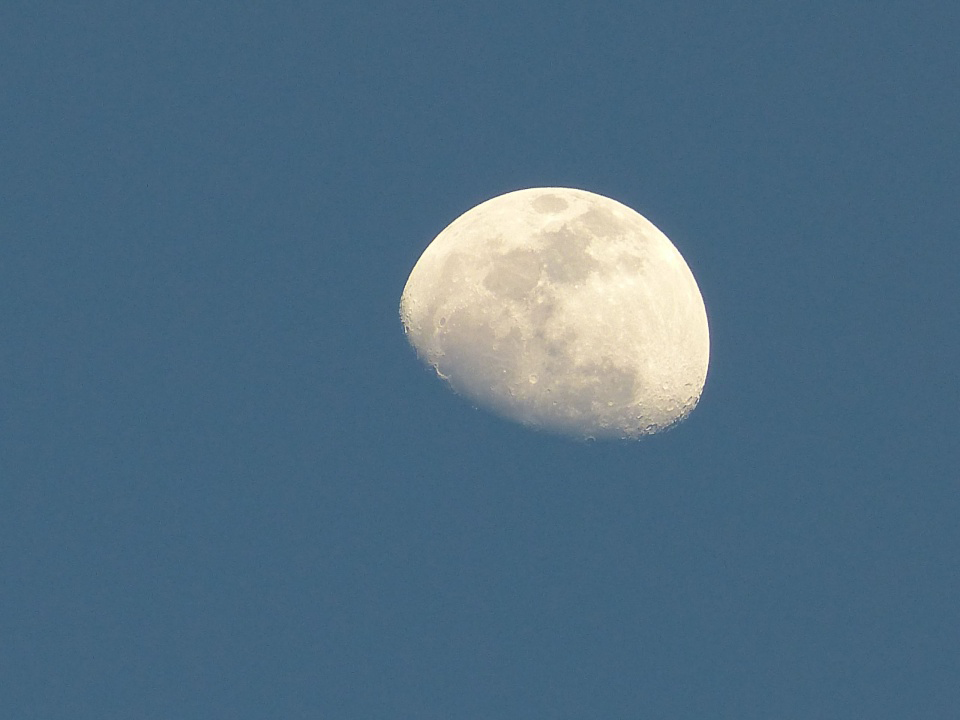
\includegraphics[width=\paperwidth,height=\paperheight]{img/title.png}
}

\frame{\titlepage}

\usebackgroundtemplate{%
    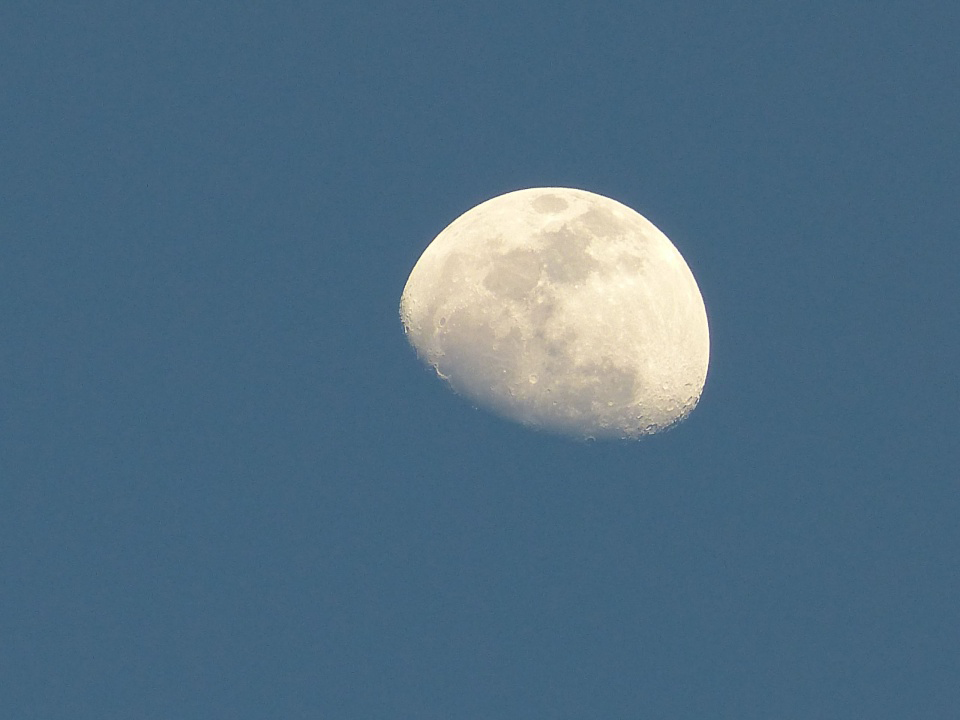
\includegraphics[width=\paperwidth,height=\paperheight]{img/content.png}
}



\section{第一章节 Tomcat 配置}



\subsection{第一小节 TomCat 参数 }

\begin{frame}
    \frametitle{第一章节 Tomcat }
    \framesubtitle{第一小节 TomCat 参数}
     \begin{itemize}
    	\item 参数配置
    	 \small
    	 
    	 -server -Xmx3000m -Xms3000m -Xmn1500m -Xss256k -XX:SurvivorRatio=6 -XX:ParallelGCThreads=8 -XX:MaxTenuringThreshold=0 -XX:+UseConcMarkSweepGC -verbose:gc -XX:+PrintGC -XX:+PrintGCDetails -XX:+PrintTenuringDistribution -XX:+PrintHeapAtGC -XX:+PrintGCTimeStamps -XX:+PrintGCDateStamps -XX:+HeapDumpOnOutOfMemoryError -Xloggc:../logs/gc.log   	
    \end{itemize}
\end{frame}


\begin{frame}
\frametitle{第一章节 Tomcat }
\framesubtitle{第一小节 TomCat 参数解释}
\begin{figure}[ht]	
	\centering
	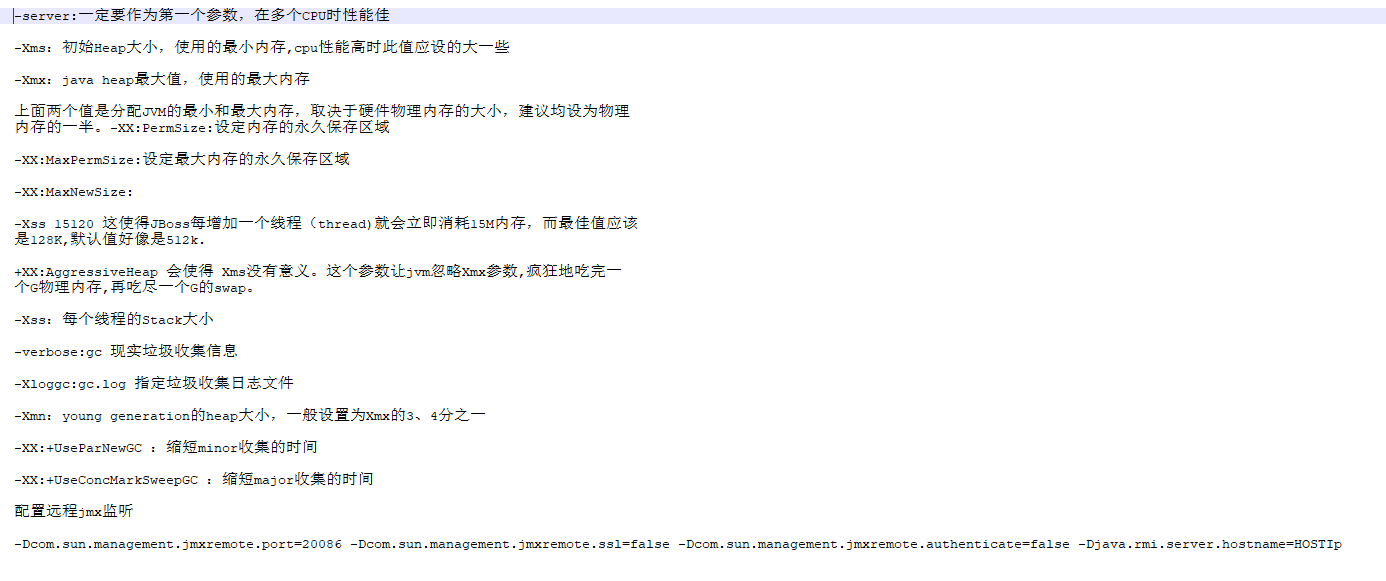
\includegraphics[scale=0.45]{img/shuoming.png}
	\caption{TomCat 参数解释}
	\label{fig:pathdemo1}
\end{figure}


\end{frame}



\subsection{第二小节 connector 参数 }

\begin{frame}
\frametitle{第一章节 Tomcat }
\framesubtitle{第二小节 connector 参数}
\begin{figure}[ht]	
	\centering
	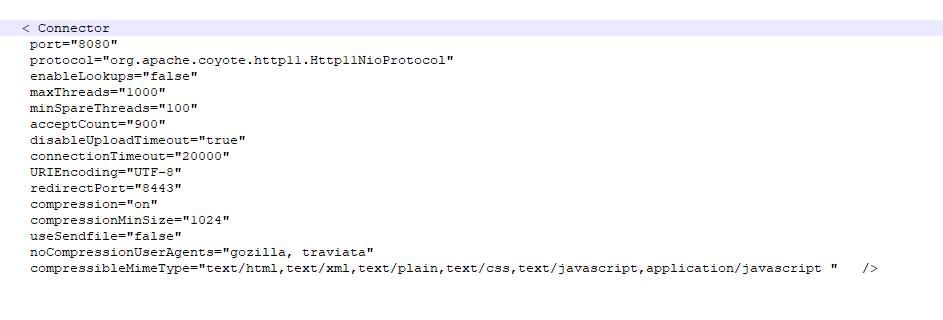
\includegraphics[scale=0.48]{img/server.png}
	\caption{connector 参数demo}
	\label{fig:pathdemo1}
\end{figure}


\end{frame}


\begin{frame}
\frametitle{第一章节 Tomcat }
\framesubtitle{第二小节 connector 参数说明}
\begin{itemize}
	
	\item 参数说明
	\small
	
	org.apache.coyote.http11.Http11NioProtocol:调整工作模式为Nio
	
	maxThreads:最大线程数,默认150。增大值避免队列请求过多,导致响应缓慢。
	
	minSpareThreads:最小空闲线程数。
	
	acceptCount:当处理请求超过此值时,将后来请求放到队列中等待。
	
	disableUploadTimeout:禁用上传超时时间
	
	connectionTimeout:连接超时,单位毫秒,0代表不限制
	
	URIEncoding:URI地址编码使用UTF-8
	
	enableLookups:关闭dns解析,提高响应时间
	
	compression:启用压缩功能
	
	compressionMinSize:最小压缩大小,单位Byte
	
	compressibleMimeType :压缩的文件类型
	
\end{itemize}
\end{frame}

\begin{frame}
\frametitle{Tomcat 总体架构图}
\begin{figure}[ht]	
	\centering
	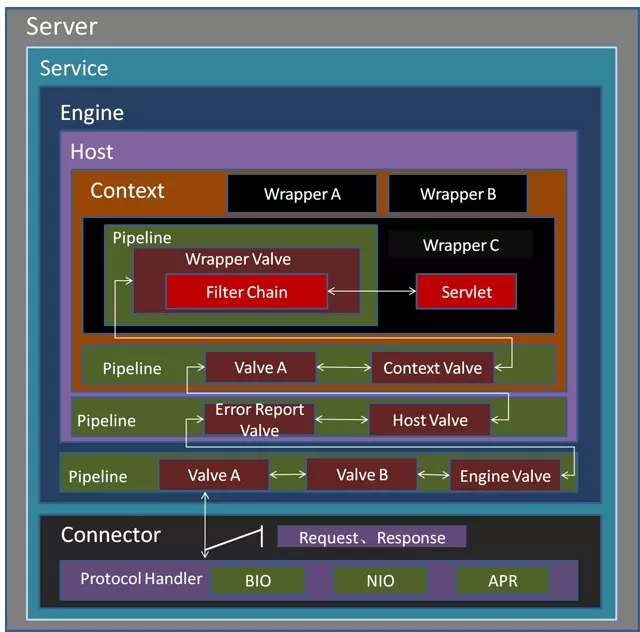
\includegraphics[scale=0.40]{img/Architect.png}
	\caption{Architect}
	\label{fig:pathdemo1}
\end{figure}

\end{frame}





\begin{frame}
\frametitle{Tomcat BIO}
\begin{figure}[ht]
	
	\centering
	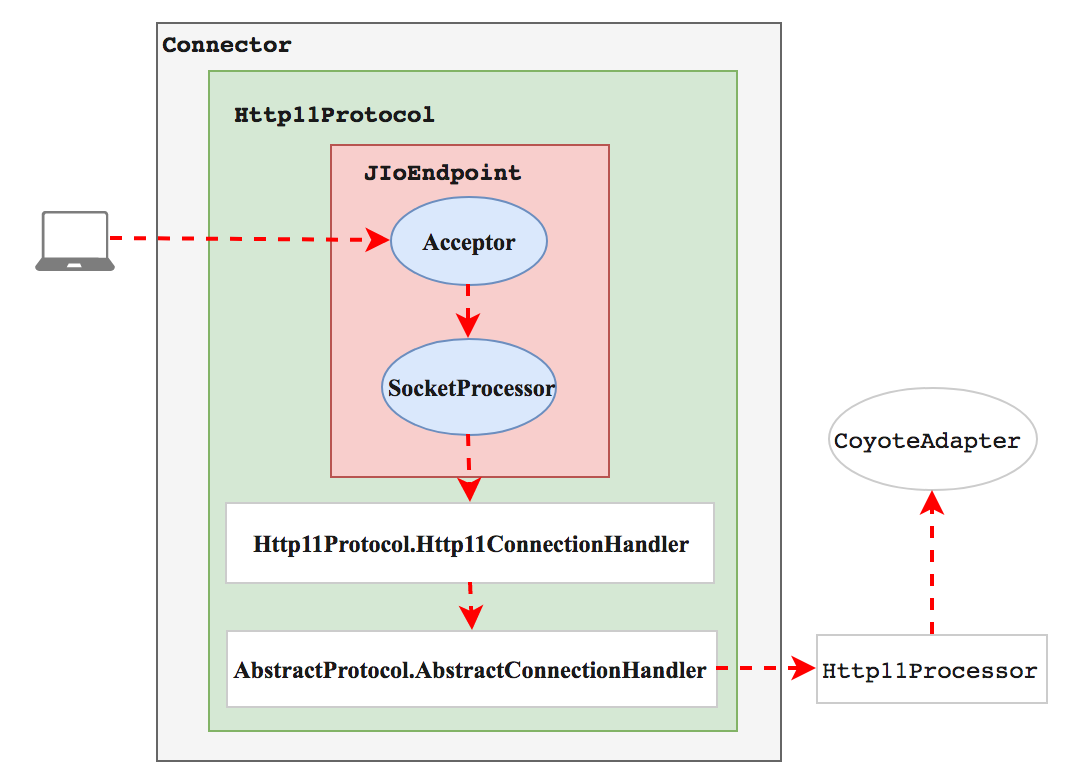
\includegraphics[scale=0.45]{img/http-BIO.png}
	\caption{http-BIO}
	\label{fig:pathdemo1}
\end{figure}

\end{frame}

\begin{frame}
\frametitle{Tomcat NIO}
\begin{figure}[ht]
	
	\centering
	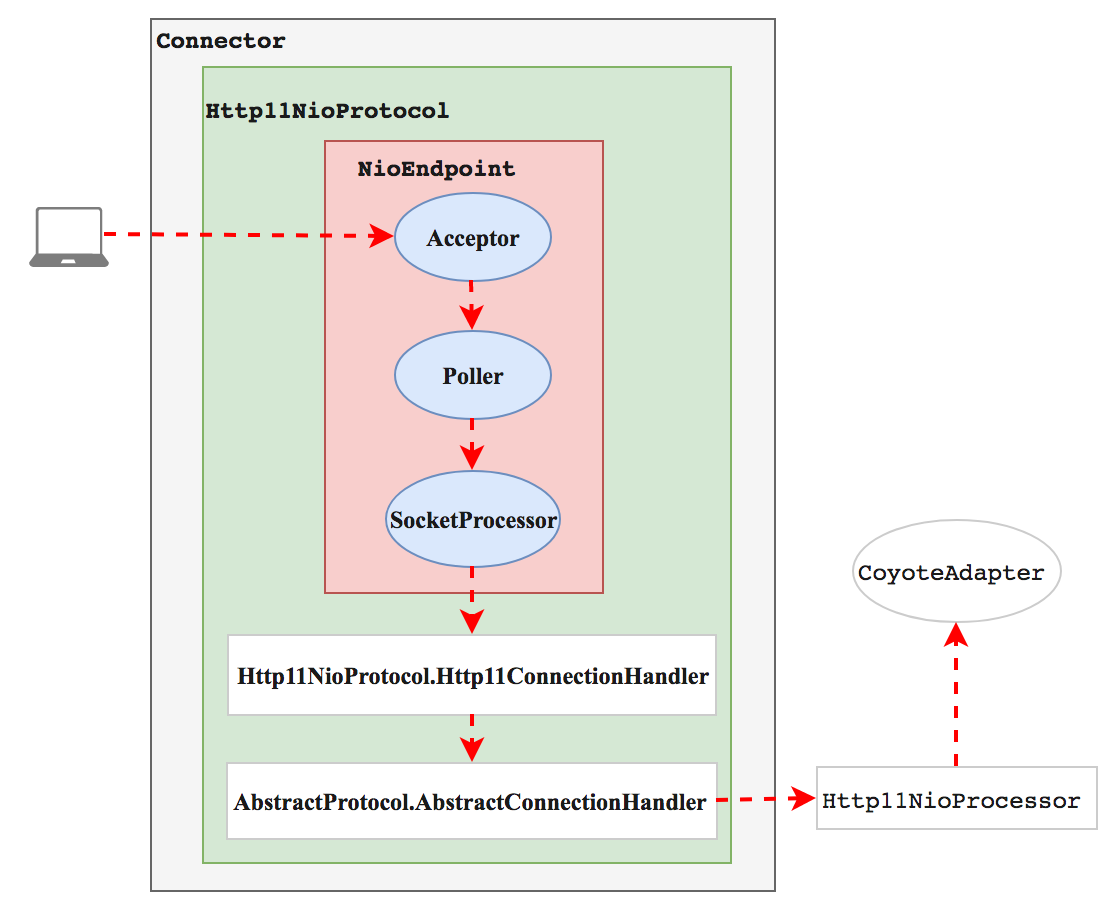
\includegraphics[scale=0.45]{img/Http-NIO.png}
	\caption{Http-NIO}
	\label{fig:pathdemo1}
\end{figure}

\end{frame}

\begin{frame}
\frametitle{Tomcat NIO2}
\begin{figure}[ht]
	
	\centering
	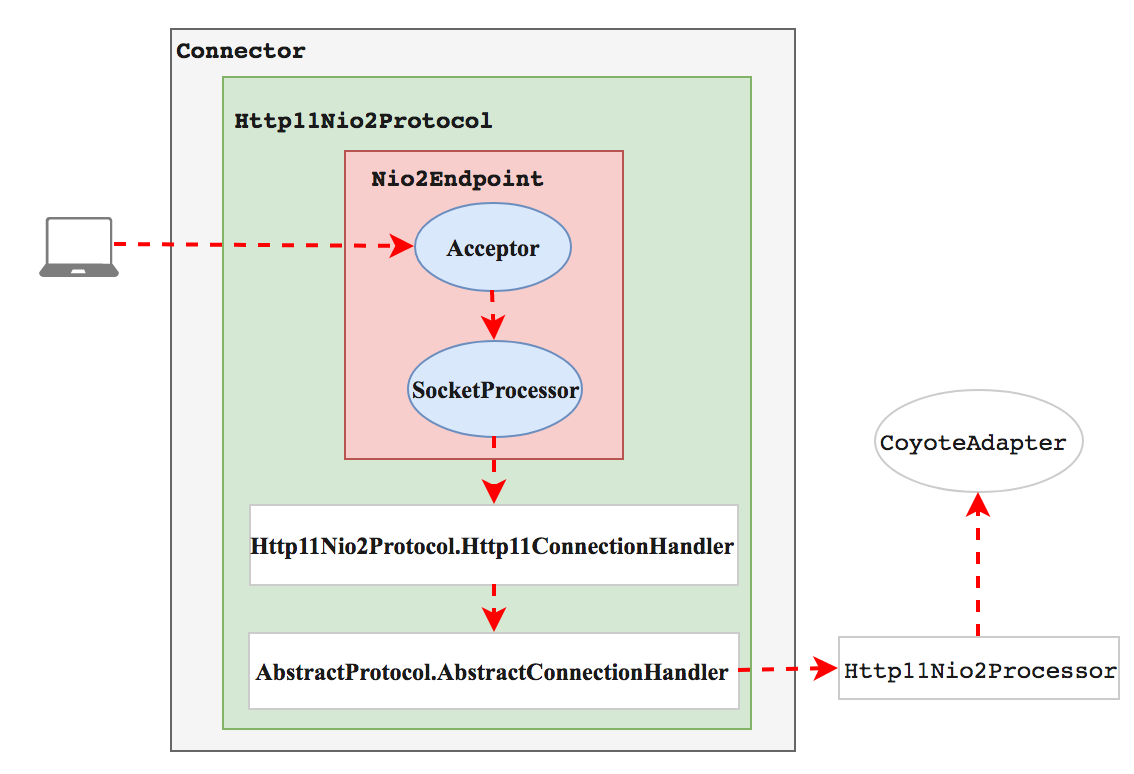
\includegraphics[scale=0.45]{img/http-NIO2.png}
	\caption{http-NIO2}
	\label{fig:pathdemo1}
\end{figure}

\end{frame}

\begin{frame}
\frametitle{Tomcat APR}
\begin{figure}[ht]
	
	\centering
	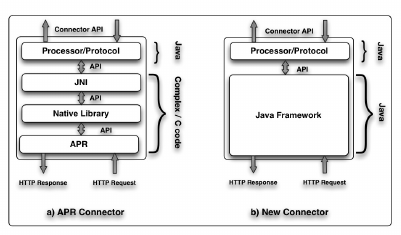
\includegraphics[scale=0.45]{img/JBoss-Web-Connector-Architecture.png}
	\caption{http-APR}
	\label{fig:pathdemo1}
\end{figure}

\end{frame}

\section{第二章节 基准测试}



\begin{frame}
\frametitle{Tomcat 基准性能}
\begin{figure}[ht]
	
	\centering
	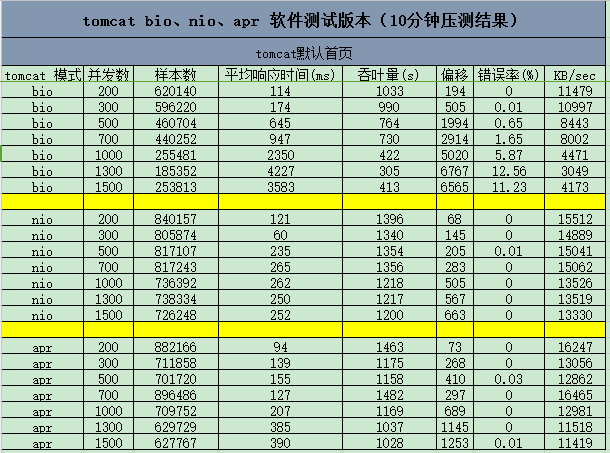
\includegraphics[scale=0.45]{img/benchmark.png}
	\caption{基准性能图表}
	\label{fig:pathdemo1}
\end{figure}

\end{frame}


\section{参考文献}

\begin{frame}[allowframebreaks]
    \frametitle{参考文献}
    \small
    \bibliographystyle{plain}
    \bibliography{slide}
    https://blog.csdn.net/mrleeapple/article/details/80420395
    
    https://zh.wikipedia.org/wiki/Apache%E5%8F%AF%E7%A7%BB%E6%A4%8D%E8%BF%90%E8%A1%8C%E6%97%B6
\end{frame}

\begin{frame}[allowframebreaks]
\frametitle{参考文献}
\centering
\begin{tabular}{|l|c|r|}
	\hline 
	\large	JDK版本 &  \large 默认GC&  \large 性能 \\
	\hline 
	JDK8 & G1非并发 &  GC \\
	\hline 
	JDK11 & G1并发 & GC \\
	\hline 
	openjdk8 & G1非并发& GC  \\
	\hline 
	openjdk11& G1并发 & GC \\
	\hline
\end{tabular}
\end{frame}

\begin{frame}[allowframebreaks]
\frametitle{JDK版本 与GC}
\centering
\begin{tabular}{|l|c|r|}
	\hline 
	\large	Connector&  \large 版本要求&  \large IO \\
	\hline 
	Http11Protocol & 7、8、9 & BIO \\
	\hline 
	Http11NioProtocol & 7、8、9 & NIO \\
	\hline 
	Http11Nio2Protocol & 8、9& NIO2  \\
	\hline 
	Http11AprProtocol& 7、8、9 & APR \\
	\hline
\end{tabular}
\end{frame}

\section*{}

\usebackgroundtemplate{%
    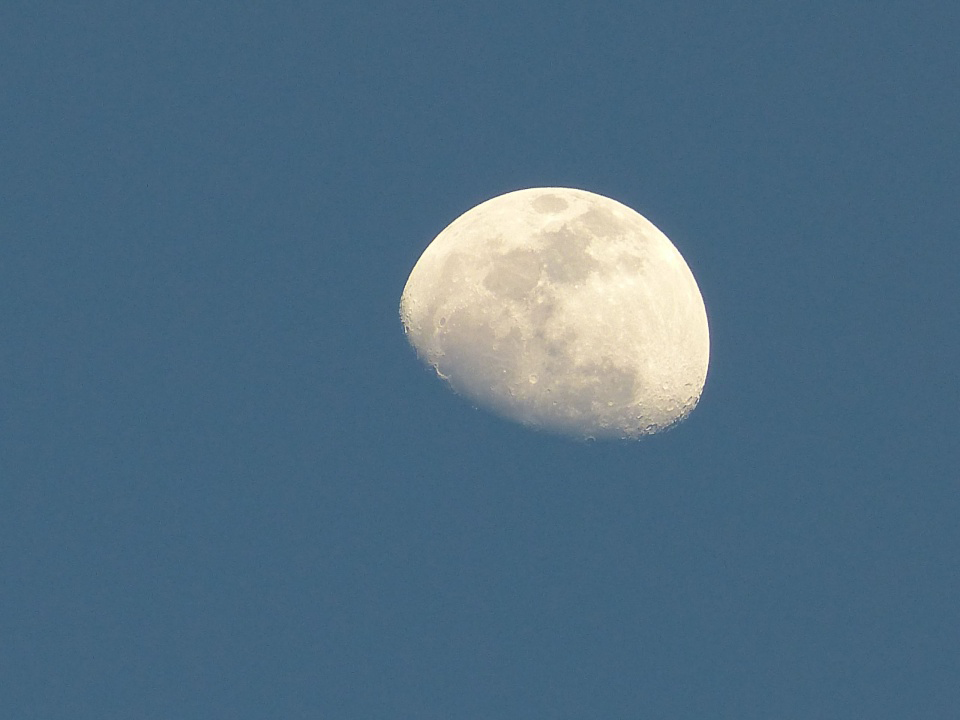
\includegraphics[width=\paperwidth,height=\paperheight]{img/title.png}
}


\begin{frame}
    \centering
   \Huge Q \& A
\end{frame}

\begin{frame}
\centering
\Huge Thank you !
\end{frame}

\end{document}
